\documentclass[11pt]{amsart}
\usepackage{geometry}                % See geometry.pdf to learn the layout options. There are lots.
\geometry{letterpaper}                   % ... or a4paper or a5paper or ... 
%\geometry{landscape}                % Activate for for rotated page geometry
%\usepackage[parfill]{parskip}    % Activate to begin paragraphs with an empty line rather than an indent
\usepackage{graphicx}
\usepackage{amssymb}
\usepackage{epstopdf}
\DeclareGraphicsRule{.tif}{png}{.png}{`convert #1 `dirname #1`/`basename #1 .tif`.png}

\usepackage{graphicx}
\graphicspath{ {images/} }

\title{Lab 3}
\author{Elise McEllhiney}
%\date{}                                           % Activate to display a given date or no date

\begin{document}
\maketitle

\section{Linear Regression}
First I normalize the inputs.  I don't necessarily have to normalize the Y values, but it made my numbers come out nicer so I normalize Y as well.  Usually I would want to just center Y but that makes the cost values large and difficult to work with.
\subsection{Gradient Descent}
If I want to retrieve the expected values from my hypotheses then I would use: $$E[Y] = \frac{h + mean}{std}$$
My gradient descent function outputs these as the finalized betas with the learning rate $\alpha = 0.01$ and the numbers of iterations $iters = 1000$
$$\beta = [ -1.10910099e-16,   8.78503652e-01,  -4.69166570e-02]$$
$$MLE=0.261406739215$$

\subsection{Ridge Gradient Descent}
The difference between regular gradient descent and ridge gradient descent is that ridge gradient descent penalizes large $\beta$ values.
My gradient descent function outputs these as the finalized betas with the learning rate $\alpha = 0.01$ and the numbers of iterations $iters = 1000$
$$\beta = [ -1.10986870e-16,   7.63060130e-01,   1.43579162e-02]$$
$$MLE = 0.271324713879$$
\begin{center}
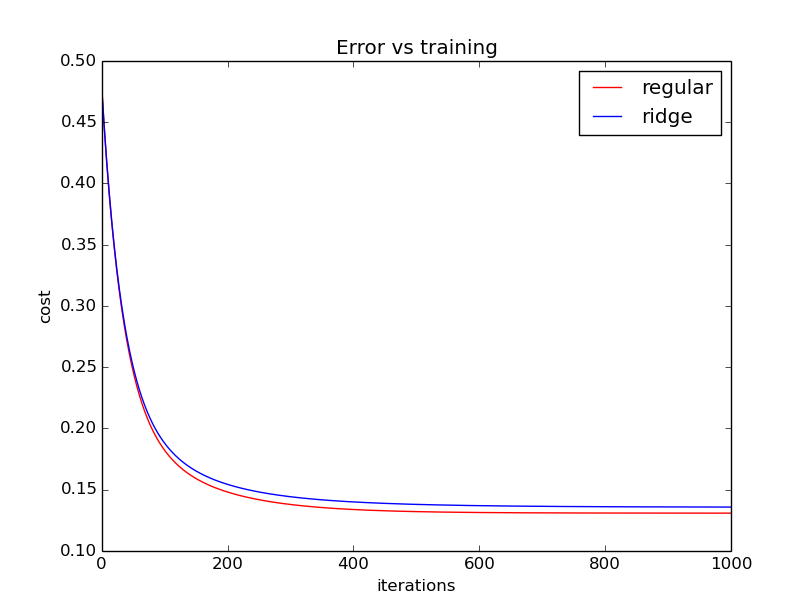
\includegraphics[scale=.75]{figure_1.png}
\end{center}
\section{Logistic Regression}
For Logistic regression I implemented the required functions and outputted as listed.  Logistic regression provides classification instead of real-number output.  My program requires that the classes are only capable of taking values of (0,1).  My regression uses $\alpha = 0.01$ and $iters = 10000$\\\\
The betas produced by my gradient descent are:: $\beta = [ 1.71844948,  4.01290252,  3.74390304]$\\
The betas acquired by the optimization function were: $\beta = [ 1.71843665,  4.01287736,  3.74387854]$\\
As you can see, these are very similar.  So, under the assumption that my gradient function works, my gradient descent also follows the optimization function.\\
My confusion matrix is as follows:\\
\begin{center}
\begin{tabular}{ l | c  r }			
   & 0 & 1 \\
   \hline
  0 & 34 & 6 \\
  1 & 5 & 55 \\
  \hline  
\end{tabular}
\end{center}
Which shows that I have an accuracy of: $89.0\%$ for this dataset 


\end{document}  